
\chapter{RESULTS AND DISCUSSIONS}

\section{{\bf{Result1}}}
{\bf\color{red}In this chapter, the author(s) shall present the results and simulations (in the form of numerical data or graphical form) of the theory described in CHAPTER-2 and finally discuss the results.
}

\section{\bf Formation of Table in \LaTeXe}


\begin{table}[htpb]
\caption{Values of parameters at different atmospheric temperatures.}
\begin{center}
\begin{tabular}{|c | c | c | c |}
\hline
Atm.Temp. & $m = M_{max}= (m_bc_b)_{max}$ & $s = S_{max}$  & $E(\times 10^{-3})$\\
$T_a\,^{\circ}\mathrm{C}$ & cal/cm$^3$-min$\,^{\circ}\mathrm{C}$ & cal/cm$^3$-min & g/cm$^2$-min\\
\hline
15 & 0.003 & 0.0357 & 0\\
23 & 0.018  & 0.018 & 0,\,0.48\\
33 & 0.0315 & 0.018 & 0.48,\,0.96\\
\hline
\end{tabular}
\end{center}
\label{tabl5.1}
\end{table}
\newpage
\subsection{\bf Subsection 1}
Your first subsection of Section 2 of Chapter 3.
\begin{figure}[htpb]
	\begin{center}
		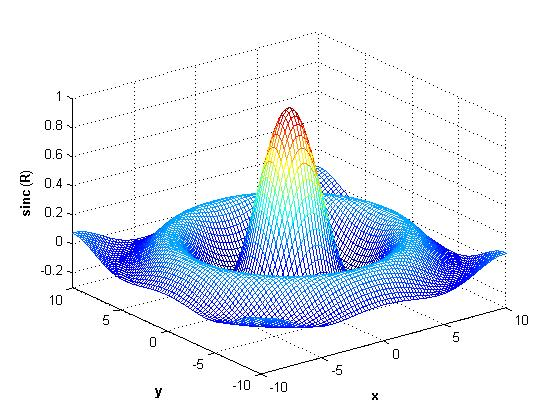
\includegraphics[height=8cm, width=8cm]{figures/msinc.jpg}
		\caption{Graph of Sinc.}
		\label{fig1.1}
	\end{center}
\end{figure}
\subsection{\bf Subsection 2}
Your second subsection of Section 2 of Chapter 3.

\begin{figure}[htpb]
\begin{center}
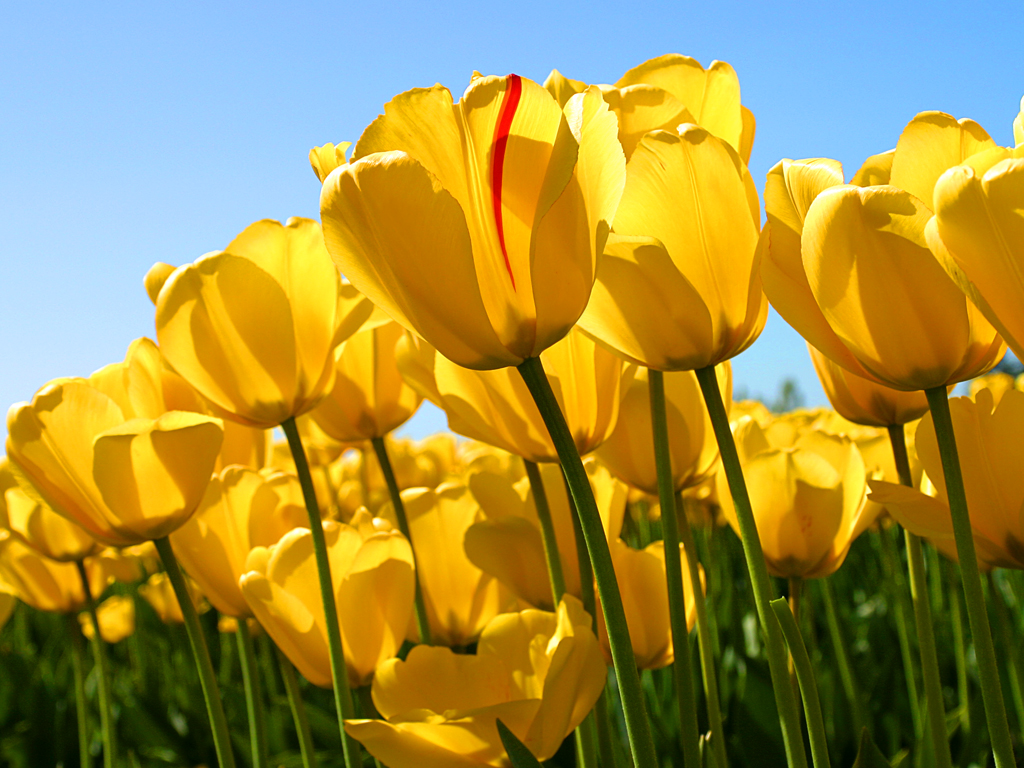
\includegraphics[height=6cm, width=6cm]{figures/Tulips.jpg}
\caption{Tulips Flower.}
\label{fig1.1}
\end{center}
\end{figure}

